%! TEX root = 'main.tex'
\section{Evaluation}
\label{sec:evaluation}

\begin{figure}[th]
	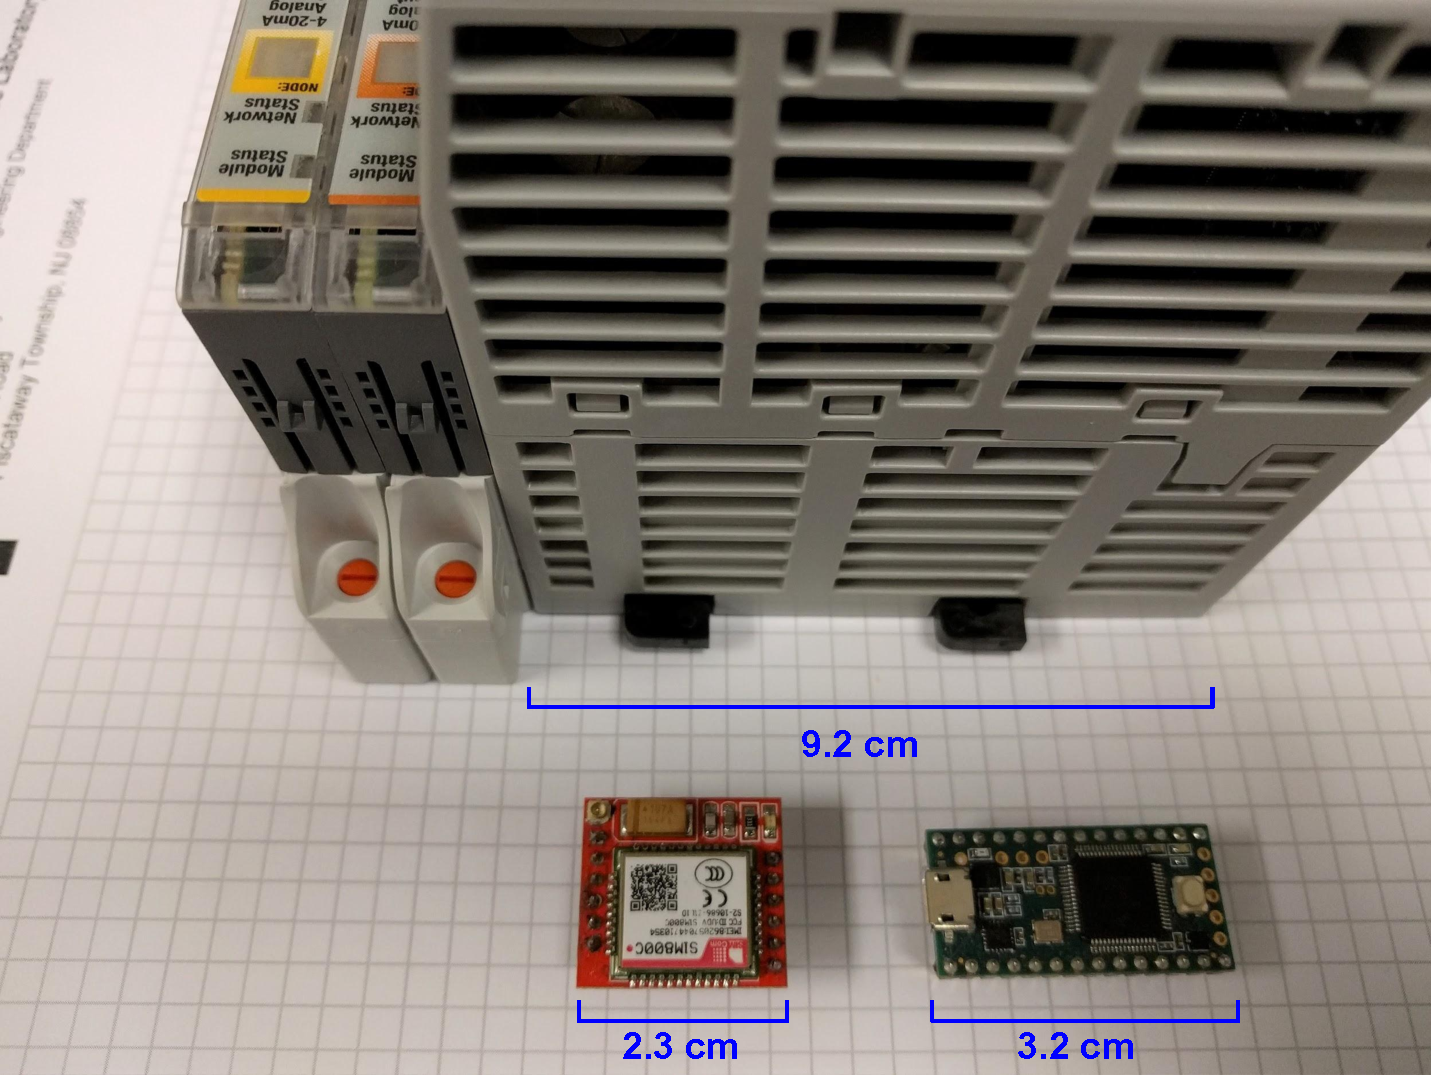
\includegraphics[width=0.47\textwidth]{figures/eval_size_old}
	\centering
	\caption{Test}
	\label{fig:eval_sizei_old}
\end{figure}

\begin{figure}[th]
	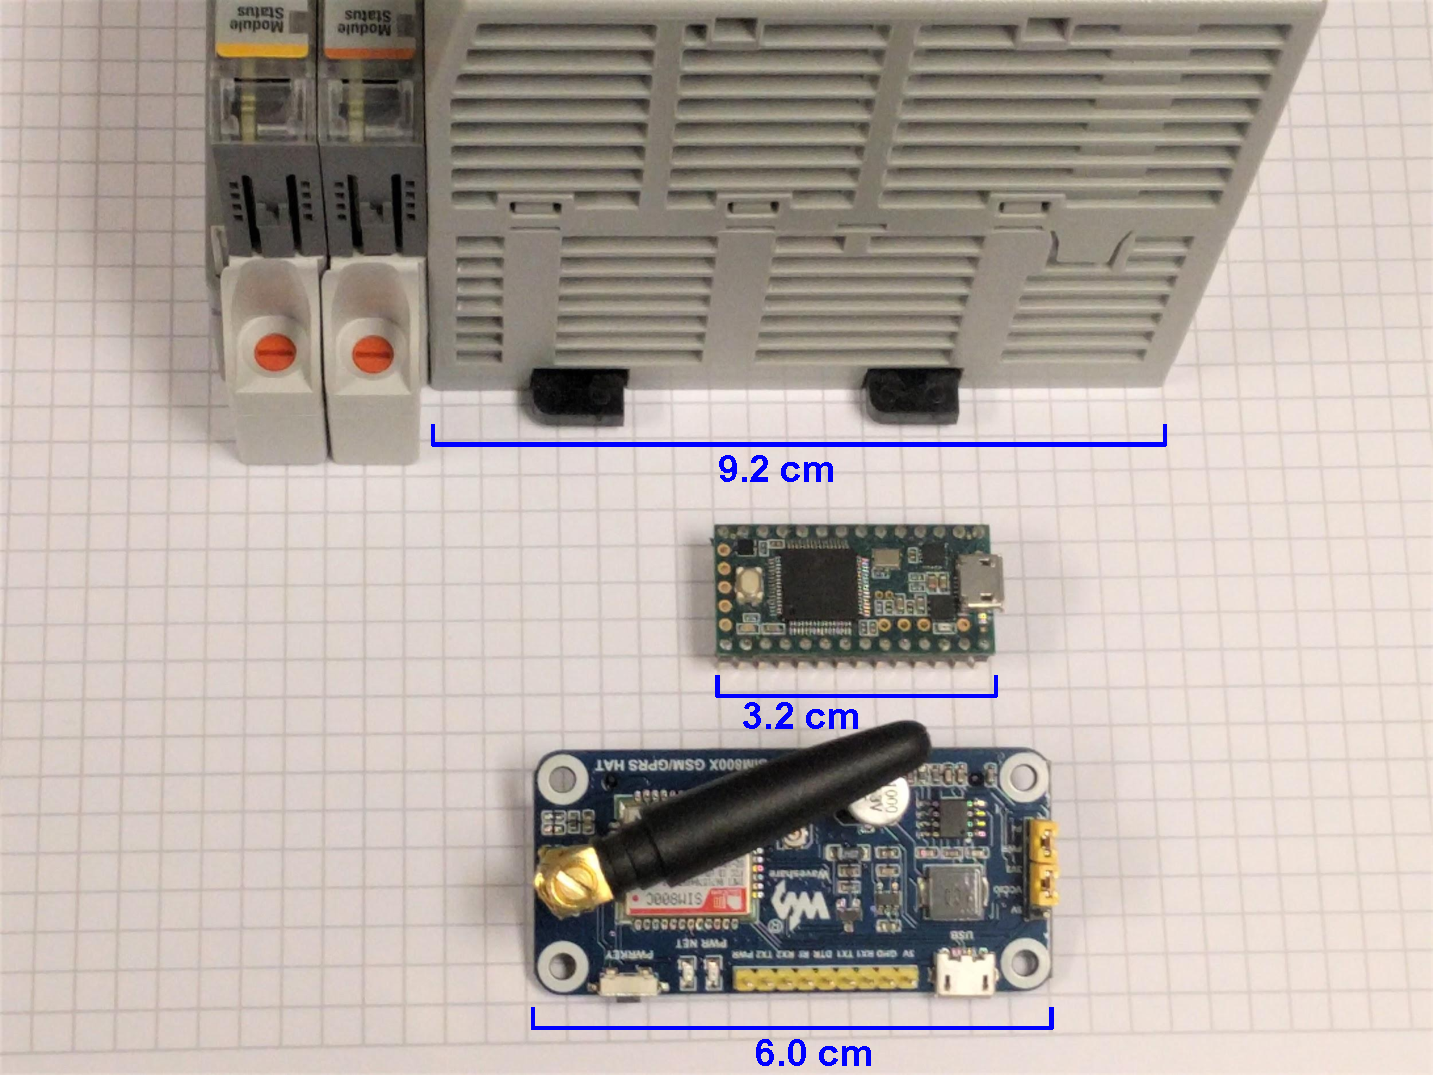
\includegraphics[width=0.47\textwidth]{figures/eval_size}
	\centering
	\caption{Test}
	\label{fig:eval_size}
\end{figure}


In our threat model, this hardware implant should exist independently of the PLC's communication network. To achieve this, as mentioned before, we chose to use cellular networks to communicate with nodes via SMS message. This approach is not as reliable as wired networks, especially in our attack model, which may require multiple nodes to launch attacks at the same time. We evaluated the approximate time required for SMS transmission, as shown in~\autoref{fig:smstime}, although we know that this may be affected by a variety of factors, such as the distance between the cell phone and the base station, the number of cell phones served by the same base station, across different networks, and so on. We also know that a SMS message over 160 characters will be split, large messages are segmented into 153 character segments and sent individually then rebuilt by the recipients device. But in order to avoid differences in the protocols implemented by different SMS programs or there may be some extra bytes attached to the SMS message, we did not strictly evaluate it by the number of SMS segments. From a practical point of view, we evaluated the transmission time corresponding to the length of the control command.

\begin{figure}[th]
	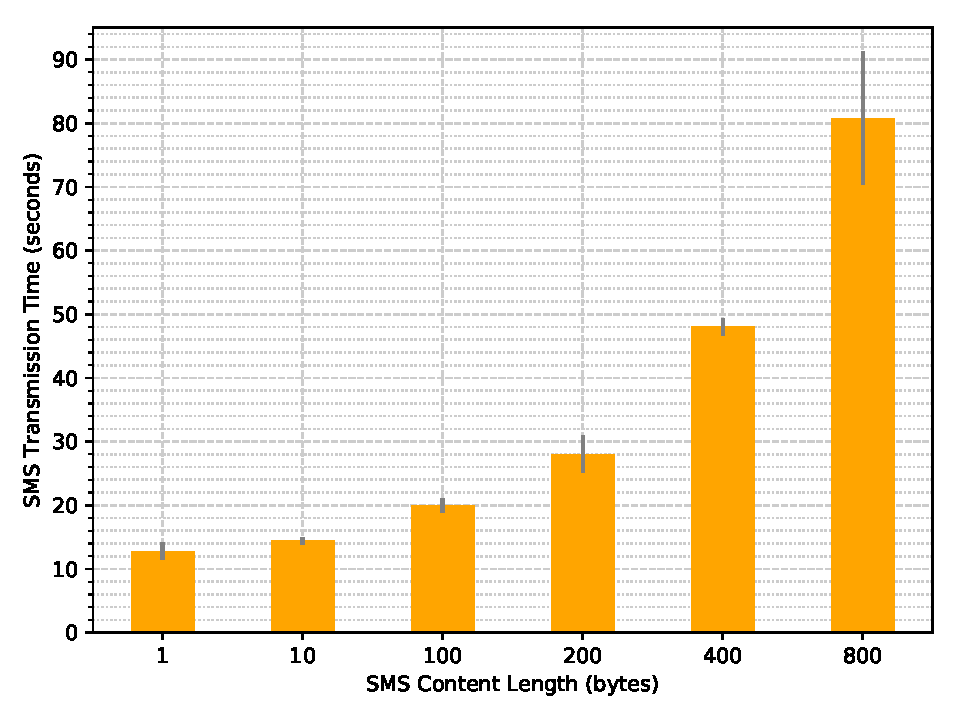
\includegraphics[width=0.47\textwidth]{figures/smstime}
	\centering
	\caption{SMS Message Transmission Time}
	\label{fig:smstime}
\end{figure}

The control command length can be only one byte, which is used to start a malicious function preset in the hardware implant. It can also be very long, such as containing a piece of binary to update the firmware of the PLC. Or it can contain a series of detailed attack instructions. The advantage of this is that even if the hardware implant is exposed, it does not contain specific attack instructions, thus avoiding further exposure to subsequence attacks and methods.

We get the data by sending a control command to a node with a phone. The command for each length was tested 20 times to obtain the mean and standard deviation. The cellular networks we used is T-Mobile and Google Fi. 

As shown in the figure, the longer the length of the control command, the more time it takes, and the less reliable it is for an attack that requires precise synchronization.

Since the payload (attack commands) is either pre-existing in the hardware implant or sent by the command message during the attack. The attack in our instance directly manipulates the output of the GPIO. So it does not need to modify any code in any PLC firmware, nor does it need to occupy the storage space of the PLC.

Due to different implementations, JTAG debugging capabilities can be intrusive or non-intrusive. The conventional JTAG debug is invasive which halt the processor using breakpoints and watchpoints. It also needs to halt the processor before it can modify any register. However, the debug functionality implemented in LM3S2793 is known as CoreSight architecture. The DAP (Debug Access Port) is an implementation of an ARM Debug Interface which provides real-time access for the debugger without halting the processor to AMBA system memory, peripheral registers and all debug configuration registers. So our hardware implant can modify the GPIO through AHB bus without any software overhead.

\begin{figure*}[h]
	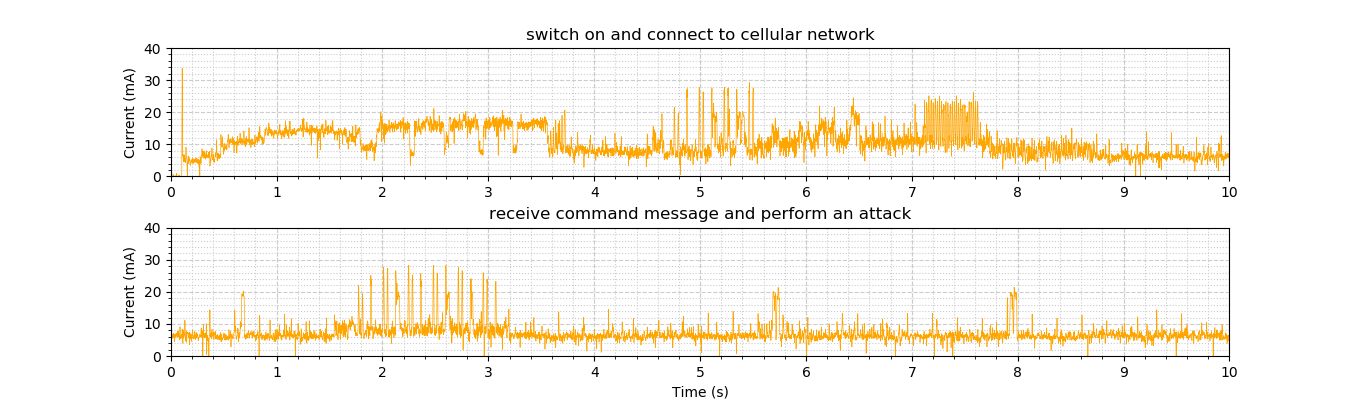
\includegraphics[width=\textwidth]{figures/current}
	\centering
	\caption{The hardware implant does not consume a lot of power, and the power consumption will only increase slightly when starting and executing the attack command. Sub-figure 1 shows the power consumption during the startup. Sub-figure 2.a shows the power consumption during an demo attack. 2.b indicates an output pin of the attacked PLC. }
	\label{fig:current}
\end{figure*}

The hardware implant is powered directly from the PLC and does not consume a lot of power. The power consumption will only increase slightly when starting and executing the attack command, as shown in~\autoref{fig:current}.

